\documentclass{beamer}


\usepackage{animate}
%\usepackage{pgfplots}
\usepackage{tikz}

\usetikzlibrary{	
	calc
}

%\RequirePackage{ifthen}

% Counters
\newcounter{m} % Number of sides of the polygon
\setcounter{m}{0}

\newcommand{\base}[1]{%
	\def\ID{#1}
	% FACILITY	
	\draw [line width=1.0,orange,fill=orange!20] (0.3,0.0) rectangle (0.8,0.5);
	\draw [line width=0.5,>=latex,->]  ( -0.1 ,  0.0 ) -- (  1.5 , 0.0 ) node [scale=0.8, below ] {$t$};
	\draw [line width=0.5,>=latex,->]  ( 0.0  , -0.1 ) -- (  0.0 , 1.0 ) node [scale=0.8, above ] {$p^{def}_{i,\ID}(t)$};
	\draw [line width=0.2,dashed]      ( 0.0  ,  0.5 ) node [scale=0.8, left ] {$P$} -- (  1.4 , 0.5 );
	\draw [line width=0.5,>=latex,<->]    ( 0.3 , -0.1 ) -- node [scale=0.8, below ] {$\tau$} (  0.8 , -0.1 ) ;
	\draw [line width=1.0,dotted, orange] ( 0.3 , -0.2 ) node[scale=0.8,below,xshift=-5,yshift=1]{$t^{act}_{i,\ID}$} -- ( 0.3 , 0.8 );
	% PDF
%	\draw [line width=0.5,>=latex,->]  ( 4.2 , 1.5 ) -- (  6.2 , 1.5 ) node [scale=0.8, below ] {$t$};
%	\draw [line width=0.5,>=latex,->]  ( 4.3 , 1.4 ) -- (  4.3 , 2.7 ) node [scale=0.8, above left ] {$pdf(t^{act}_{i,j})$};	
%	\draw [line width=0.5           ]  plot[smooth, raw gnuplot] function{ plot "pv_grid_profile" u (($0)*1.5/23 + 4.5):(($1)+1.5) };
%	\draw [line width=0.2,dashed    ]  ( 4.5 , 1.4 ) node [scale=0.5, below ] {$t^{beg}_{i,j}$} -- (  4.5 , 2.5 );	
%	\draw [line width=0.2,dashed    ]  ( 6.0 , 1.4 ) node [scale=0.5, below ] {$t^{end}_{i,j}$} -- (  6.0 , 2.5 );		
	%MAIN GRAPH
	\draw [line width=0.5,black,fill=black!20] (2.5,-2.0) rectangle (2.7,-1.8);
	\draw [line width=0.5,black,fill=black!20] (2.5,-1.8) rectangle (2.7,-1.6);
	\draw [line width=0.5,black,fill=black!20] (2.5,-1.6) rectangle (2.7,-1.4);
	\draw [line width=0.5,black,fill=black!20] (2.5,-1.4) rectangle (2.7,-1.2);	
	\draw [line width=0.5,black,fill=black!20] (2.7,-2.0) rectangle (2.9,-1.8);
	\draw [line width=0.5,black,fill=black!20] (2.7,-1.8) rectangle (2.9,-1.6);
	\draw [line width=0.5,black,fill=black!20] (2.7,-1.6) rectangle (2.9,-1.4);	
	\draw [line width=0.5,black,fill=black!20] (2.9,-2.0) rectangle (3.1,-1.8);
	\draw [line width=0.5,black,fill=black!20] (2.9,-1.8) rectangle (3.1,-1.6);		
	\draw [line width=0.5,black,fill=black!20] (3.1,-2.0) rectangle (3.3,-1.8);	
	\draw [line width=0.5,black,fill=black!20] (3.3,-2.0) rectangle (3.5,-1.8);	
	\draw [line width=0.5,black,fill=black!20] (3.5,-2.0) rectangle (3.7,-1.8);	
	\draw [line width=0.5,black,fill=black!20] (3.7,-2.0) rectangle (3.9,-1.8);
	\draw [line width=0.5,black,fill=black!20] (3.7,-1.8) rectangle (3.9,-1.6);
	\draw [line width=0.5,black,fill=black!20] (3.7,-1.6) rectangle (3.9,-1.4);	

	\draw [line width=0.5, dashed]     plot[smooth, raw gnuplot] function{plot "pv_grid_profile" u (($0)*3.0/24 + 2.5):(($1) - 2.2)};	
	\draw [line width=0.5,>=latex,->]  ( 2.4 , -2.0 ) -- (  5.5 , -2.0 ) node [scale=0.8, below ] {$t$};
	\draw [line width=0.5,>=latex,->]  ( 2.5 , -2.1 ) -- (  2.5 , -0.5 ) node [scale=1.0, above ] {$p^{c}_{i}(t)$};
	\draw [line width=1.0,dotted, orange] ( 3.9 , -2.2 ) node[scale=0.8,below]{$t^{beg}_{i,\ID}$} -- ( 3.9 , -1.0 );
	\draw [line width=1.0,dotted, orange] ( 4.7 , -2.2 ) node[scale=0.8,below]{$t^{end}_{i,\ID}$} -- ( 4.7 , -1.0 );
%	\draw [line width=2.0,orange,>=latex,->]  ( 1.6 ,  0.5 ) to[out=0,in=100] (  4.0 , -1.0 );
}


\begin{document}

\begin{frame}

\begin{animateinline}[autoplay,loop,width=0.9\textwidth]{10}

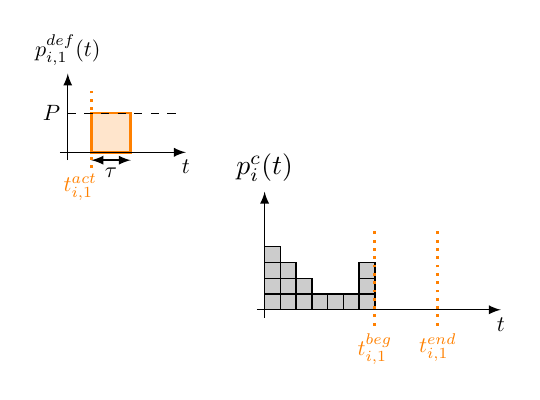
\begin{tikzpicture}
	\base{1}
\end{tikzpicture}
\newframe

\multiframe{11}{rPos=0+0.1}{
	\begin{tikzpicture}
	\base{1}
	% ELIPSE EQUATION: (x/a)^2 + (y/b)^2 = 1
	\pgfmathparse{ 2.6 * \rPos }\let\xp = \pgfmathresult
	\pgfmathparse{ ( 2.5 * sqrt( 1 - ( \xp / 2.6 )^2 ) ) }\let\yp = \pgfmathresult
	\pgfmathparse{ \xp + 1.5 }\let\xpos = \pgfmathresult
	\pgfmathparse{ \yp - 2.0 }\let\ypos = \pgfmathresult
	\draw [line width=0.5,orange,fill=orange!20] (\xpos,\ypos) rectangle ({\xpos + 0.2},{\ypos + 0.2});	
	\end{tikzpicture}
}
\newframe

\multiframe{11}{rPos=0+0.1}{
	\begin{tikzpicture}
	\base{2}
	\draw [line width=0.5,orange,fill=orange!20] (4.1,-2.0) rectangle (4.3,-1.8);
	% ELIPSE EQUATION: (x/a)^2 + (y/b)^2 = 1
	\pgfmathparse{ 2.8 * \rPos }\let\xp = \pgfmathresult
	\pgfmathparse{ ( 2.5 * sqrt( 1 - ( \xp / 2.8 )^2 ) ) }\let\yp = \pgfmathresult
	\pgfmathparse{ \xp + 1.5 }\let\xpos = \pgfmathresult
	\pgfmathparse{ \yp - 2.0 }\let\ypos = \pgfmathresult
	\draw [line width=0.5,orange,fill=orange!20] (\xpos,\ypos) rectangle ({\xpos + 0.2},{\ypos + 0.2});	
	\end{tikzpicture}
}
\newframe

\multiframe{11}{rPos=0+0.1}{
	\begin{tikzpicture}
	\base{3}
	\draw [line width=0.5,orange,fill=orange!20] (4.1,-2.0) rectangle (4.3,-1.8);
	\draw [line width=0.5,orange,fill=orange!20] (4.3,-2.0) rectangle (4.5,-1.8);
	% ELIPSE EQUATION: (x/a)^2 + (y/b)^2 = 1
	\pgfmathparse{ 2.6 * \rPos }\let\xp = \pgfmathresult
	\pgfmathparse{ ( 2.3 * sqrt( 1 - ( \xp / 2.6 )^2 ) ) }\let\yp = \pgfmathresult
	\pgfmathparse{ \xp + 1.5 }\let\xpos = \pgfmathresult
	\pgfmathparse{ \yp - 1.8 }\let\ypos = \pgfmathresult
	\draw [line width=0.5,orange,fill=orange!20] (\xpos,\ypos) rectangle ({\xpos + 0.2},{\ypos + 0.2});	
	\end{tikzpicture}
}
\newframe

\multiframe{11}{rPos=0+0.1}{
	\begin{tikzpicture}
	\base{4}
	\draw [line width=0.5,orange,fill=orange!20] (4.1,-2.0) rectangle (4.3,-1.8);
	\draw [line width=0.5,orange,fill=orange!20] (4.1,-1.8) rectangle (4.3,-1.6);
	\draw [line width=0.5,orange,fill=orange!20] (4.3,-2.0) rectangle (4.5,-1.8);
	% ELIPSE EQUATION: (x/a)^2 + (y/b)^2 = 1
	\pgfmathparse{ 2.4 * \rPos }\let\xp = \pgfmathresult
	\pgfmathparse{ ( 2.5 * sqrt( 1 - ( \xp / 2.4 )^2 ) ) }\let\yp = \pgfmathresult
	\pgfmathparse{ \xp + 1.5 }\let\xpos = \pgfmathresult
	\pgfmathparse{ \yp - 2.0 }\let\ypos = \pgfmathresult
	\draw [line width=0.5,orange,fill=orange!20] (\xpos,\ypos) rectangle ({\xpos + 0.2},{\ypos + 0.2});	
	\end{tikzpicture}
}
\newframe

\multiframe{11}{rPos=0+0.1}{
	\begin{tikzpicture}
	\base{5}
	\draw [line width=0.5,orange,fill=orange!20] (3.9,-2.0) rectangle (4.1,-1.8);
	\draw [line width=0.5,orange,fill=orange!20] (4.1,-2.0) rectangle (4.3,-1.8);
	\draw [line width=0.5,orange,fill=orange!20] (4.1,-1.8) rectangle (4.3,-1.6);
	\draw [line width=0.5,orange,fill=orange!20] (4.3,-2.0) rectangle (4.5,-1.8);
	% ELIPSE EQUATION: (x/a)^2 + (y/b)^2 = 1
	\pgfmathparse{ 2.4 * \rPos }\let\xp = \pgfmathresult
	\pgfmathparse{ ( 2.3 * sqrt( 1 - ( \xp / 2.4 )^2 ) ) }\let\yp = \pgfmathresult
	\pgfmathparse{ \xp + 1.5 }\let\xpos = \pgfmathresult
	\pgfmathparse{ \yp - 1.8 }\let\ypos = \pgfmathresult
	\draw [line width=0.5,orange,fill=orange!20] (\xpos,\ypos) rectangle ({\xpos + 0.2},{\ypos + 0.2});	
	\end{tikzpicture}
}
\newframe

\multiframe{11}{rPos=0+0.1}{
	\begin{tikzpicture}
	\base{6}
	\draw [line width=0.5,orange,fill=orange!20] (3.9,-2.0) rectangle (4.1,-1.8);
	\draw [line width=0.5,orange,fill=orange!20] (3.9,-1.8) rectangle (4.1,-1.6);
	\draw [line width=0.5,orange,fill=orange!20] (4.1,-2.0) rectangle (4.3,-1.8);
	\draw [line width=0.5,orange,fill=orange!20] (4.1,-1.8) rectangle (4.3,-1.6);
	\draw [line width=0.5,orange,fill=orange!20] (4.3,-2.0) rectangle (4.5,-1.8);
	% ELIPSE EQUATION: (x/a)^2 + (y/b)^2 = 1
	\pgfmathparse{ 2.4 * \rPos }\let\xp = \pgfmathresult
	\pgfmathparse{ ( 2.1 * sqrt( 1 - ( \xp / 2.4 )^2 ) ) }\let\yp = \pgfmathresult
	\pgfmathparse{ \xp + 1.5 }\let\xpos = \pgfmathresult
	\pgfmathparse{ \yp - 1.6 }\let\ypos = \pgfmathresult
	\draw [line width=0.5,orange,fill=orange!20] (\xpos,\ypos) rectangle ({\xpos + 0.2},{\ypos + 0.2});	
	\end{tikzpicture}
}
\newframe

\multiframe{11}{rPos=0+0.1}{
	\begin{tikzpicture}
	\base{7}
	\draw [line width=0.5,orange,fill=orange!20] (3.9,-2.0) rectangle (4.1,-1.8);
	\draw [line width=0.5,orange,fill=orange!20] (3.9,-1.8) rectangle (4.1,-1.6);
	\draw [line width=0.5,orange,fill=orange!20] (3.9,-1.6) rectangle (4.1,-1.4);
	\draw [line width=0.5,orange,fill=orange!20] (4.1,-2.0) rectangle (4.3,-1.8);
	\draw [line width=0.5,orange,fill=orange!20] (4.1,-1.8) rectangle (4.3,-1.6);
	\draw [line width=0.5,orange,fill=orange!20] (4.3,-2.0) rectangle (4.5,-1.8);
	% ELIPSE EQUATION: (x/a)^2 + (y/b)^2 = 1
	\pgfmathparse{ 3.0 * \rPos }\let\xp = \pgfmathresult
	\pgfmathparse{ ( 2.5 * sqrt( 1 - ( \xp / 3.0 )^2 ) ) }\let\yp = \pgfmathresult
	\pgfmathparse{ \xp + 1.5 }\let\xpos = \pgfmathresult
	\pgfmathparse{ \yp - 2.0 }\let\ypos = \pgfmathresult
	\draw [line width=0.5,orange,fill=orange!20] (\xpos,\ypos) rectangle ({\xpos + 0.2},{\ypos + 0.2});		
	\end{tikzpicture}
}
\newframe

\multiframe{11}{rPos=0+0.1}{
	\begin{tikzpicture}
	\base{8}
	\draw [line width=0.5,orange,fill=orange!20] (3.9,-2.0) rectangle (4.1,-1.8);
	\draw [line width=0.5,orange,fill=orange!20] (3.9,-1.8) rectangle (4.1,-1.6);
	\draw [line width=0.5,orange,fill=orange!20] (3.9,-1.6) rectangle (4.1,-1.4);
	\draw [line width=0.5,orange,fill=orange!20] (4.1,-2.0) rectangle (4.3,-1.8);
	\draw [line width=0.5,orange,fill=orange!20] (4.1,-1.8) rectangle (4.3,-1.6);
	\draw [line width=0.5,orange,fill=orange!20] (4.3,-2.0) rectangle (4.5,-1.8);
	\draw [line width=0.5,orange,fill=orange!20] (4.5,-2.0) rectangle (4.7,-1.8);
	% ELIPSE EQUATION: (x/a)^2 + (y/b)^2 = 1
	\pgfmathparse{ 2.4 * \rPos }\let\xp = \pgfmathresult
	\pgfmathparse{ ( 1.9 * sqrt( 1 - ( \xp / 2.4 )^2 ) ) }\let\yp = \pgfmathresult
	\pgfmathparse{ \xp + 1.5 }\let\xpos = \pgfmathresult
	\pgfmathparse{ \yp - 1.4 }\let\ypos = \pgfmathresult
	\draw [line width=0.5,orange,fill=orange!20] (\xpos,\ypos) rectangle ({\xpos + 0.2},{\ypos + 0.2});	
	\end{tikzpicture}
}


\end{animateinline}

\end{frame}

\end{document}


























